\documentclass{oblivoir}
%%%Default packages
\usepackage{amsmath,amssymb,amsthm,kotex,tabu,graphicx,pifont}
\usepackage{../kswrapfig}

\usepackage{gensymb} %\degree

%%%More packages
%\usepackage{caption,subcaption}
%\usepackage[perpage]{footmisc}
%
\usepackage[skipabove=10pt,innertopmargin=10pt,nobreak=true]{mdframed}

\usepackage[inline]{enumitem}
\setlist[enumerate,1]{label=(\arabic*)}
\setlist[enumerate,2]{label=(\alph*)}

\usepackage{multicol}
\setlength{\columnsep}{30pt}
\setlength{\columnseprule}{1pt}
%
%\usepackage{forest}
%\usetikzlibrary{shapes.geometric,arrows.meta,calc}
%
%%%defi theo exam prob rema proo
%이 환경들 아래에 문단을 쓸 경우 살짝 들여쓰기가 되므로 \hspace{-.7em}가 필요할 수 있다.

\newcounter{num}
\newcommand{\defi}[1]
{\noindent\refstepcounter{num}\textbf{정의 \arabic{num})} #1\par\noindent}
\newcommand{\theo}[1]
{\noindent\refstepcounter{num}\textbf{정리 \arabic{num})} #1\par\noindent}
\newcommand{\revi}[1]
{\noindent\refstepcounter{num}\textbf{복습 \arabic{num})} #1\par\noindent}
\newcommand{\exam}[1]
{\bigskip\bigskip\noindent\refstepcounter{num}\textbf{예시 \arabic{num})} #1\par\noindent}
\newcommand{\prob}[1]
{\bigskip\bigskip\noindent\refstepcounter{num}\textbf{문제 \arabic{num})} #1\par\noindent}
\newcommand{\rema}[1]
{\bigskip\bigskip\noindent\refstepcounter{num}\textbf{참고 \arabic{num})} #1\par\noindent}
\newcommand{\proo}
{\bigskip\noindent\textsf{증명)}}

\newenvironment{talign}
 {\let\displaystyle\textstyle\align}
 {\endalign}
\newenvironment{talign*}
 {\let\displaystyle\textstyle\csname align*\endcsname}
 {\endalign}
%
%%%Commands

\newcommand{\procedure}[1]{\begin{mdframed}\vspace{#1\textheight}\end{mdframed}}

\newcommand\an[1]{\par\bigskip\noindent\textbf{문제 \ref{#1})}\par\noindent}

\newcommand\ann[2]{\par\bigskip\noindent\textbf{문제 \ref{#1})}\:\:#2\par\medskip\noindent}

\newcommand\ans[1]{\begin{flushright}\textbf{답 : }#1\end{flushright}}

\newcommand\anssec[1]{\bigskip\bigskip\noindent{\large\bfseries#1}}

\newcommand{\pb}[1]%\Phantom + fBox
{\fbox{\phantom{\ensuremath{#1}}}}

\newcommand\ba{\,|\,}

\newcommand\ovv[1]{\ensuremath{\overline{#1}}}
\newcommand\ov[2]{\ensuremath{\overline{#1#2}}}
%
%%%% Settings
%\let\oldsection\section
%
%\renewcommand\section{\clearpage\oldsection}
%
%\let\emph\textsf
%
%\renewcommand{\arraystretch}{1.5}
%
%%%% Footnotes
%\makeatletter
%\def\@fnsymbol#1{\ensuremath{\ifcase#1\or
%*\or **\or ***\or
%\star\or\star\star\or\star\star\star\or
%\dagger\or\dagger\dagger\or\dagger\dagger\dagger
%\else\@ctrerr\fi}}
%
%\renewcommand{\thefootnote}{\fnsymbol{footnote}}
%\makeatother
%
%\makeatletter
%\AtBeginEnvironment{mdframed}{%
%\def\@fnsymbol#1{\ensuremath{\ifcase#1\or
%*\or **\or ***\or
%\star\or\star\star\or\star\star\star\or
%\dagger\or\dagger\dagger\or\dagger\dagger\dagger
%\else\@ctrerr\fi}}%
%}   
%\renewcommand\thempfootnote{\fnsymbol{mpfootnote}}
%\makeatother
%
%%% 객관식 선지
\newcommand\one{\ding{172}}
\newcommand\two{\ding{173}}
\newcommand\three{\ding{174}}
\newcommand\four{\ding{175}}
\newcommand\five{\ding{176}}
\usepackage{tabto,pifont}
%\TabPositions{0.2\textwidth,0.4\textwidth,0.6\textwidth,0.8\textwidth}

\newcommand\taba[5]{\par\noindent
\one\:{#1}
\tabto{0.2\textwidth}\two\:\:{#2}
\tabto{0.4\textwidth}\three\:\:{#3}
\tabto{0.6\textwidth}\four\:\:{#4}
\tabto{0.8\textwidth}\five\:\:{#5}}

\newcommand\tabb[5]{\par\noindent
\one\:{#1}
\tabto{0.33\textwidth}\two\:\:{#2}
\tabto{0.67\textwidth}\three\:\:{#3}\medskip\par\noindent
\four\:\:{#4}
\tabto{0.33\textwidth}\five\:\:{#5}}

\newcommand\tabc[5]{\par\noindent
\one\:{#1}
\tabto{0.5\textwidth}\two\:\:{#2}\medskip\par\noindent
\three\:\:{#3}
\tabto{0.5\textwidth}\four\:\:{#4}\medskip\par\noindent
\five\:\:{#5}}

\newcommand\tabd[5]{\par\noindent
\one\:{#1}\medskip\par\noindent
\two\:\:{#2}\medskip\par\noindent
\three\:\:{#3}\medskip\par\noindent
\four\:\:{#4}\medskip\par\noindent
\five\:\:{#5}}
%
%%%% fonts
%
%\usepackage{fontspec, xunicode, xltxtra}
%\setmainfont[]{은 바탕}
%\setsansfont[]{은 돋움}
%\setmonofont[]{은 바탕}
%\XeTeXlinebreaklocale "ko"
%%%%
\begin{document}

\title{수학(하) : 08 집합}
\author{}
\date{\today}
\maketitle
\tableofcontents
\newpage

%%sets
\section{집합과 원소}

%
\exam{}
\begin{enumerate}\label{sets1}
\item
`어떤 조건이나 기준에 의하여 그 대상을 분명히 알 수 있는 것들의 모임'을 \emph{집합}이라고 한다.
또, 집합을 이루는 대상 하나하나를 \emph{원소}라고 한다.
\item
예를 들어 `\(6\)의 약수의 모임', `성북구에 위치한 초등학교의 모임'은 집합이다.
하지만 `\(6\)에 가까운 수들의 모임', `착한 학생들이 다니는 초등학교의 모임'은 집합이 아니다.
\item
원소가 하나도 없는 집합을 \emph{공집합}이라고 하고 기호로는  \(\varnothing\)로 나타낸다.
\item
\(A\)를 `\(6\)의 약수의 모임'이라고 하자.
그러면 \(2\)는 \(A\)의 원소이다.
이것을
\[2\in A\]
으로 표현한다.
반면 \(4\)는 \(A\)의 원소가 아니다.
이것을
\[4\notin A\]
으로 표현한다.
마찬가지로 \(B\)를 `성북구에 위치한 초등학교의 모임'이라고 하면
\[\text{일신초등학교}\in B\]
이고
\[\text{영훈초등학교}\notin B\]
이다.
\item
\(A\)의 원소에는 \(1\), \(2\), \(3\), \(6\)의 네 개가 있다.
이것을
\[A=\{1,2,3,6\}\]
으로 표현한다.
혹은
\[A=\{x\ba x\text{는 6의 약수}\}\]
으로 표현하기도 한다.
\end{enumerate}

%
\begin{mdframed}
\defi{원소나열법, 조건제시법}\label{sets2}
\[A=\{1,2,3,6\}\]
와 같이 표현하는 방법을 `원소나열법'이라고 한다.
\[A=\{x\ba x\text{는 6의 약수}\}\]
와 같이 표현하는 방법을 `조건제시법'이라고 한다.
\end{mdframed}

%
\prob{}
\begin{enumerate}\label{sets3}
\item
\(10\)보다 작은 자연수의 모임		\tabto{0.6\textwidth}(집합이다, 집합이 아니다)
\item
큰 수들의 모임							\tabto{0.6\textwidth}(집합이다, 집합이 아니다)
\item
\(2\)보다 작은 소수의 모임			\tabto{0.6\textwidth}(집합이다, 집합이 아니다)
\item
예쁘게 생긴 꽃들의 모임				\tabto{0.6\textwidth}(집합이다, 집합이 아니다)
\item
키가 \(170\)cm 이상인 학생들의 모임	\tabto{0.6\textwidth}(집합이다, 집합이 아니다)
\end{enumerate}

%
\prob{}\label{sets4}
\(A\)를 `\(10\)보다 작은 소수들의 모임'이라고 할 때, 다음 빈 칸에 \(\in\), \(\notin\) 중 알맞은 기호를 써넣어라.
\\[10pt]
\begin{enumerate*}[itemjoin={,\qquad\qquad}]
\item
\(1\:\:\pb{\in}\:\:A\)
\item
\(3\:\:\pb{\in}\:\:A\)
\item
\(7\:\:\pb{\in}\:\:A\)
\item
\(9\:\:\pb{\in}\:\:A\)
\end{enumerate*}

%
\prob{}\label{sets5}
\(B\)가 `\(18\)의 약수들의 집합'일 때, \(B\)를 원소나열법과 조건제시법으로 나타내어라.

%
\prob{}\label{sets6}
\(C\)가 `\(4\)의 배수들의 모임'일 때, \(C\)를 원소나열법과 조건제시법으로 나타내어라.

%%subset
\section{부분집합}
%
\exam{}
\begin{enumerate}\label{subset1}
\item
\(A=\{1,3,5\}\), \(B=\{1,2,3,4,5\}\)이라고 하자.
이것을 그림\footnotemark으로
\footnotetext{이러한 그림을 벤 다이어그램(Venn Diagram)이라고 부른다.}
\begin{center}
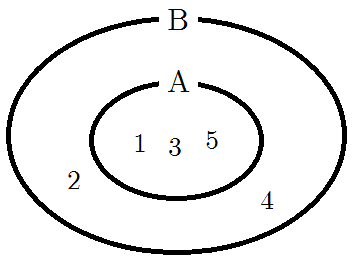
\includegraphics[width=0.27\textwidth]{subset_1}
\end{center}
와 같이 나타낼 수 있다.
이처럼 \(A\)가 \(B\)안에 포함되면
\footnote{정확하게는 ``집합 \(A\)의 모든 원소가 집합 \(B\)에 포함되면''}
\[A\subset B\]
로 나타내고 `\(A\)가 \(B\)의 부분집합이다'라고 말한다.
\item
\(A=\{2,3,4\}\), \(B=\{3,4,5\}\)이면
\begin{center}
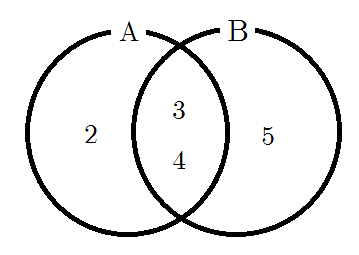
\includegraphics[width=0.25\textwidth]{subset_2}
\end{center}
이다.
\(A\)는 \(B\)에 포함되지 않고 \(B\)도 \(A\)에 포함되지 않으므로
\[A\not\subset B,\qquad B\not\subset A\]
이다.
\item
만약 두 집합 \(A\), \(B\)가 \(A\subset B\)이고 \(B\subset A\)이면
\[A=B\]
로 나타내고 `집합 \(A\), \(B\)가 같다'고 말한다.
\item
만약 두 집합 \(A\), \(B\)가 \(A\subset B\)이고 \(A\neq B\)이면
\[A\subsetneq B\]
로 나타내고 `\(A\)가 \(B\)의 \emph{진부분집합}이다'라고 말한다.
\end{enumerate}

%
\prob{}\label{subset2}
\(\subset\), \(=\)을 사용하여 \(A\)와 \(B\) 사이의 포함관계를 나타내어라.

\begin{enumerate}
\item
\(A=\{x\ba x\text{는 3의 약수}\}\), \tabto{0.48\textwidth}\(B=\{x\ba x\text{는 6의 약수}\}\)
\item
\(A=\{x\ba x\text{는 3의 배수}\}\), \tabto{0.48\textwidth}\(B=\{x\ba x\text{는 6의 배수}\}\)
\item
\(A=\{x\ba x^2-4x+3=0\}\), \tabto{0.48\textwidth}\(B=\{1,3\}\)
\end{enumerate}

%
\prob{}\label{subset3}
다음 중 틀린 것을 고르시오.
\tabd
{\(\{2,4\}\)는 \(\{2,4,6\}\)의 부분집합이다.}
{\(\{2,4\}\)는 \(\{2,4,6\}\)의 진부분집합이다.}
{\(\{2,4\}\)는 \(\{2,4\}\)의 부분집합이다.}
{\(\{2,4\}\)는 \(\{2,4\}\)의 진부분집합이다.}
{\(\{2,4\}=\{4,2\}\)이다.}

%
\prob{}\label{subset4}
두 집합 \(A=\{2,3,5,7\}\), \(B=\{4,5,6,7,8\}\)를 벤다이어그램으로 나타내어라.

%
\section{부분집합의 개수}

%
\exam{}\label{ssubset1}
집합 \(B=\{a,b\}\)의 부분집합을 모두 구하고, 그 개수를 말하여라.
\begin{mdframed}
\(\varnothing\subset B\),\quad \(\{a\}\subset B\),\quad \(\{b\}\subset B\),\quad \(\{a,b\}\subset B\)
이므로\\ \(B\)의 부분집합의 개수는 4개이다.
\end{mdframed}
\ans{\(\varnothing\), \(\{a\}\), \(\{b\}\), \(\{a,b\}\); 4개}

%
\prob{}\label{ssubset2}
다음 집합들의 부분집합을 모두 구하고, 그 개수를 말하여라.
\begin{enumerate}
\item
\(A=\{a\}\)
\item
\(C=\{a,b,c\}\)
\item
\(D=\{a,b,c,d\}\)
\end{enumerate}

%
\prob{}\label{ssubset3}
예시 \ref{ssubset1})과 문제 \ref{ssubset2})로부터
다음 집합들의 부분집합의 개수를 유추하여라.
\begin{enumerate}
\item
\(E=\{a,b,c,d,e\}\)
\item
\(F=\{a,b,c,d,e,f\}\)
\end{enumerate}

%
\begin{mdframed}
\theo{}\label{ssubset4}
원소의 개수가 \(k\)개인 집합의 부분집합의 개수는 \pb{2^k}개이다.
\end{mdframed}

%
\prob{}\label{ssubset5}
\(P=\{1,3,5,7\}\)일 때, \(P\)의 부분집합의 개수를 구하여라.

\newpage
%
\exam{집합 \(C=\{a,b,c\}\)에 대하여 다음 물음에 답하여라.}
\begin{enumerate}\label{ssubset6}
\item
\(a\)를 원소로 가지지 않는 부분집합의 개수를 구하여라.
\item
\(a\)를 원소로 가지는 부분집합의 개수를 구하여라.
\end{enumerate}

\begin{mdframed}[skipabove=0pt]
\(C\)의 부분집합은
\[\varnothing,\:\{a\},\:\{b\},\:\{c\},\:\{a,b\},\:\{a,c\},\:\{b,c\},\:\{a,b,c\}\]
의 \(8\)개가 있다.
이중 \(a\)를 원소로 가지지 않는 부분집합은
\[\varnothing,\:\{b\},\:\{c\},\:\{b,c\}\]
의 4개이고, \(a\)를 를 원소로 가지는 부분집합은
\[\{a\},\:\{a,b\},\:\{a,c\},\:\{a,b,c\}\]
의 4개이다.
\end{mdframed}
\ans{(1) \(4\)개,\qquad (2) \(4\)개}

%
\prob{}\label{ssubset7}
집합 \(D=\{a,b,c,d\}\)에 대하여 다음 물음에 답하여라.
\begin{enumerate}
\item
\(a\)를 원소로 가지지 않는 부분집합의 개수를 구하여라.
\item
\(a\)를 원소로 가지는 부분집합의 개수를 구하여라.
\item
\(a,b\)를 원소로 가지지 않는 부분집합의 개수를 구하여라.
\item
\(a,b\)를 원소로 가지는 부분집합의 개수를 구하여라.
\end{enumerate}

%
\begin{mdframed}
\theo{\normalfont{원소의 개수가 \(k\)개인 집합의 부분집합 중}}
\begin{enumerate}\label{ssubset8}
\item
\(m\)개를 원소로 가지지 않는 것의 개수는 \pb{2^{k-m}}개이다.
\item
\(m\)개를 원소로 가지는 것의 개수는 \pb{2^{k-m}}개이다.
\end{enumerate}
\end{mdframed}


%%opreations
\section{집합의 연산}
%
\exam{합집합, 교집합, 차집합}
\begin{minipage}{0.65\textwidth}\label{operations1}
(1)\:\(A=\{1,2,3,4\}\), \(B=\{4,5,6\}\)일 때, 이것을 벤다이어그램으로 표현하면 오른쪽 그림과 같다.
\end{minipage}
\begin{minipage}{0.3\textwidth}
\begin{center}
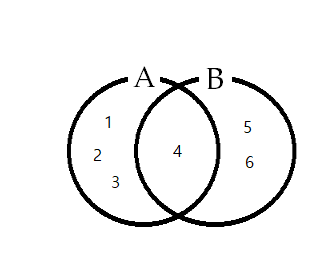
\includegraphics[width=\textwidth]{operations_1-1}
\end{center}
\end{minipage}

\noindent
\begin{minipage}{0.65\textwidth}
(2)\:\(A\)와 \(B\)를 합친 부분을
\(A\)와 \(B\)의 \emph{합집합}이라고 부르고 기호로 \(A\cup B\)로 표현한다.
따라서
\[A\cup B=\{1,2,3,4,5,6\}\]
\end{minipage}
\begin{minipage}{0.3\textwidth}
\begin{center}
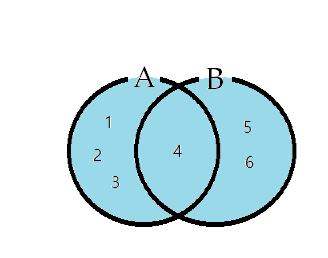
\includegraphics[width=\textwidth]{operations_1-2}
\end{center}
\end{minipage}

\noindent
\begin{minipage}{0.65\textwidth}
(3)\:\(A\)와 \(B\)를 겹치는 부분을
\(A\)와 \(B\)의 \emph{교집합}이라고 부르고 기호로 \(A\cap B\)로 표현한다.
따라서
\[A\cap B=\{4\}\]
\end{minipage}
\begin{minipage}{0.3\textwidth}
\begin{center}
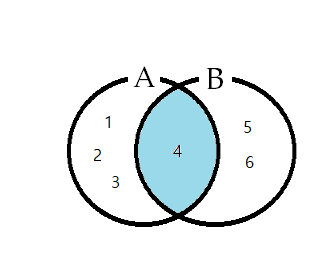
\includegraphics[width=\textwidth]{operations_1-3}
\end{center}
\end{minipage}

\noindent
\begin{minipage}{0.65\textwidth}
(4)\:\(A\)에만 해당되고 \(B\)에는 해당되지 않는 부분을
\(A\)에 대한 \(B\)의 \emph{차집합}이라고 부르고 기호로 \(A-B\)로 표현한다.
따라서
\[A-B=\{1,2,3\}\]
또한 반대로 생각하면
\[B-A=\{5,6\}\]
이다.
\end{minipage}
\begin{minipage}{0.3\textwidth}
\begin{center}
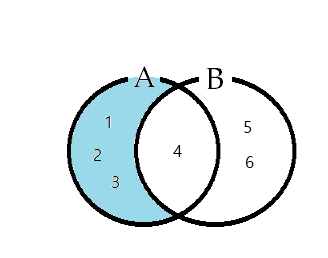
\includegraphics[width=\textwidth]{operations_1-4}\\
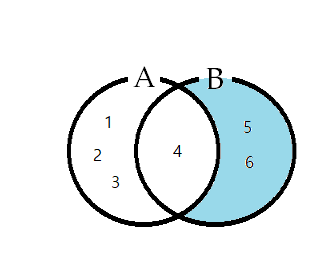
\includegraphics[width=\textwidth]{operations_1-5}\\
\end{center}
\end{minipage}

\newpage
%
\begin{mdframed}
\defi{합집합, 교집합, 차집합}\label{operations2}
두 집합 \(A\), \(B\)에 대하여
\begin{align*}
A\cup B&=\{x\ba x\in A\text{ 또는 }x\in B\}\\
A\cap B&=\{x\ba x\in A\text{ 그리고 }x\in B\}\\
A-B&=\{x\ba x\in A\text{ 그리고 }x\notin B\}
\end{align*}
\end{mdframed}

%
\prob{}\label{operations3}
다음 두 집합 \(A\), \(B\)에 대해 \(A\cup B\), \(A\cap B\), \(A-B\), \(B-A\)를 구하여라.
\begin{enumerate}
\item
\(A=\{1,3,5,7,9\}\), \(B=\{2,3,5,7\}\)
\item
\(A=\{x\ba x\text{는 }6\text{의 약수}\}\), \(B=\{x\ba x\text{는 }12\text{의 약수}\}\)
\end{enumerate}

%
\prob{}\label{operations4}
세 집합 \(A=\{1,4,7,10\}\), \(B=\{2,4,6,8,10\}\), \(C=\{4,5,7,9\}\)에 대하여 다음을 차례대로 구하여라.
\par\medskip\noindent
\begin{enumerate*}[itemjoin={\tabto{0.5\textwidth}}]
\item
\(B\cup C\)
\item
\(A\cup(B\cup C)\)
\end{enumerate*}

\begin{mdframed}
%
\defi{서로소}
두 집합 \(A\)와 \(B\)에 대해, \(A\)와 \(B\)가 공통된 원소를 가지고 있지 않으면, 즉
\[A\cap B=\varnothing\]
이면, `\(A\), \(B\)가 \textbf{서로소}이다'라고 한다.
\end{mdframed}

%
\prob{}
세 집합
\[A=\{5,10\},\quad B=\{1,3,5,7,9\},\quad C=\{1,4,7\}\]
중에서 서로소인 두 집합을 찾아라.

\newpage
%
\exam{여집합}\label{operations5}
\begin{minipage}{0.65\textwidth}
(1)\:전체집합 \(U=\{x\ba x\text{는 \(10\) 이하의 자연수}\}\)와\\ \(U\)의 부분집합 \(A\)를 
\[A=\{3,6,9\}\]
라고 하자.
\end{minipage}
\begin{minipage}{0.3\textwidth}
\begin{center}
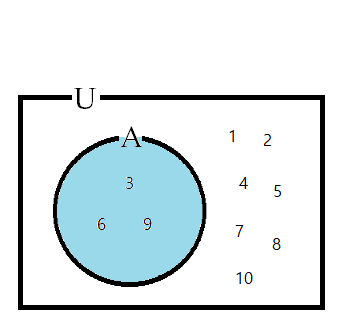
\includegraphics[width=\textwidth]{operations_5-1}
\end{center}
\end{minipage}

\noindent
\begin{minipage}{0.65\textwidth}
(2)\:이때, \(A\)의 바깥쪽에 있는 부분을 \(A\)의 \emph{여집합}이라고 부르고 기호로 \(A^c\)로 표현한다.
따라서
\[A^c=\{1,2,4,5,7,8,10\}\]
\end{minipage}
\begin{minipage}{0.3\textwidth}
\begin{center}
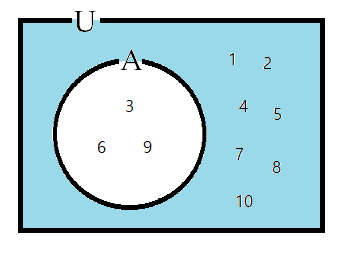
\includegraphics[width=\textwidth]{operations_5-2}
\end{center}
\end{minipage}

%
\begin{mdframed}
\defi{여집합}\label{operations6}
전체집합 \(U\)의 부분집합 \(A\)에 대하여
\[A^c=\{x\ba x\in U\text{ 그리고 }x\notin A\}\]
이다.
즉 \(A^c=U-A\)이다.
\end{mdframed}

%
\exam{}\label{operations7}
\begin{minipage}{0.65\textwidth}
(1)\:한편, \(B\)를 \(B=\{2,4,6,8,10\}\)이라고 하면
\[B^c=\{1,3,5,7,9\}\]
이다.
\end{minipage}
\begin{minipage}{0.3\textwidth}
\begin{center}
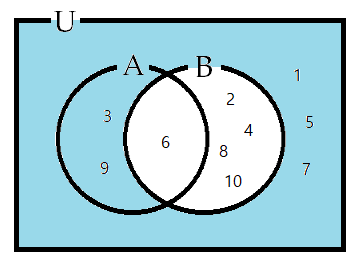
\includegraphics[width=\textwidth]{operations_5-3}
\end{center}
\end{minipage}

\noindent
\begin{minipage}{0.65\textwidth}
(2)\:따라서 \(A\cap B^c\)는
\[A\cap B^c=\{3,9\}\]
이다.
즉
\[A-B=A\cap B^c\]
이 성립한다.
\end{minipage}
\begin{minipage}{0.3\textwidth}
\begin{center}
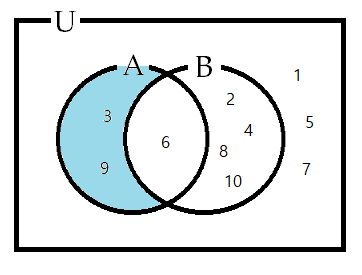
\includegraphics[width=\textwidth]{operations_5-4}
\end{center}
\end{minipage}

%
\begin{mdframed}
\theo{차집합의 성질}\label{operations8}
두 집합 \(A\), \(B\)에 대하여
\[A-B=A\cap B^c\]
이다.
\end{mdframed}

%
\prob{}\label{operations9}
전체집합 \(U=\{x\ba x\text{는 7 이하의 자연수}\}\)의 두 부분집합
\[A=\{1,2,3,4,5\},\quad B=\{1,4,7\}\]
에 대하여 \(A^c\), \(B^c\), \(A\cap B^c\)를 구하여라.

%%
%\prob{}\label{operations10}
%전체집합 \(U=\{x\ba x\text{는 10 이하의 자연수}\}\)의 두 부분집합
%\[A=\{x\ba x\text{는 10 이하의 짝수}\},\quad B=\{x\ba x\text{는 10 이하의 소수}\}\]
%에 대하여 \(A\cup B\), \((A\cup B)^c\), \(A\cap B\), \((A\cap B)^c\)를 구하여라.

%
\prob{집합 \(A\)에 대하여 다음 중 틀린 것을 고르시오.}\label{operations11}
\par\noindent
\begin{minipage}{0.65\textwidth}
\tabd
{\((A^c)^c=A\)}
{\(\varnothing^c=U\)}
{\(A\cap\varnothing=\varnothing\)}
{\(A\cup U=\varnothing\)}
{\(A\)와 \(A^c\)는 서로소이다.}
\end{minipage}
\begin{minipage}{0.3\textwidth}
\begin{center}
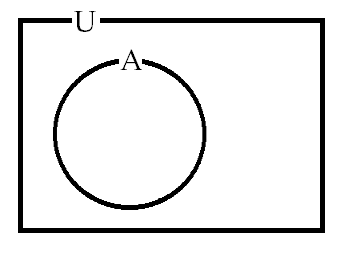
\includegraphics[width=\textwidth]{operations_11}
\end{center}
\end{minipage}

%%properties
\section{집합의 연산법칙}

%
\begin{mdframed}
\theo{집합의 연산법칙}
\begin{enumerate}\label{properties1}
\item
\(A\cup B=B\cup A\)
\tabto{0.67\textwidth}[교환법칙]\\
\(A\cap B=B\cap A\)
\item
\((A\cup B)\cup C=A\cup(B\cup C)\)
\tabto{0.67\textwidth}[결합법칙]\\
\((A\cap B)\cap C=A\cap(B\cap C)\)
\item
\(A\cup(B\cap C)=(A\cup B)\cap(A\cup C)\)
\tabto{0.67\textwidth}[분배법칙]\\
\(A\cap(B\cup C)=(A\cap B)\cup(A\cap C)\)
\item
\(A-B=A\cap B^c\)
\tabto{0.67\textwidth}[차집합의 성질]
\item
\((A\cup B)^c=A^c\cap B^c\)
\tabto{0.67\textwidth}[드 모르간의 법칙]\\
\((A\cap B)^c=A^c\cup B^c\)
\end{enumerate}
\end{mdframed}

%
\exam{교환법칙}
\begin{minipage}{0.65\textwidth}\label{properties2}
(1)\:\(A=\{2,4,5,7,9\}\), \(B=\{5,6,7,8\}\)이라고 하면
\begin{align*}
A\cup B&=\{2,4,5,6,7,8,9\}\\
B\cup A&=\{2,4,5,6,7,8,9\}
\end{align*}
이다.
즉
\[A\cup B=B\cup A\]
\end{minipage}
\begin{minipage}{0.3\textwidth}
\begin{center}
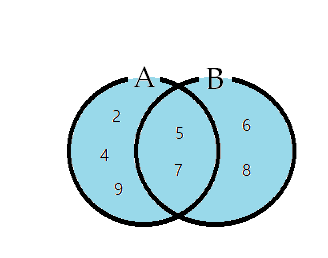
\includegraphics[width=\textwidth]{properties_2-1}
\end{center}
\end{minipage}

\bigskip\bigskip\noindent
\begin{minipage}{0.65\textwidth}
(2)\:또한
\begin{align*}
A\cap B&=\{5,7\}\\
B\cap A&=\{5,7\}
\end{align*}
이다.
즉
\[A\cap B=B\cap A\]
\end{minipage}
\begin{minipage}{0.3\textwidth}
\begin{center}
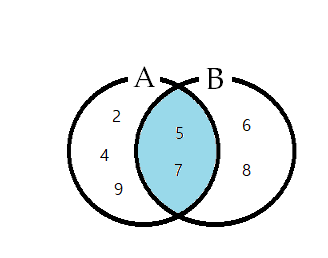
\includegraphics[width=\textwidth]{properties_2-2}
\end{center}
\end{minipage}

\newpage
%
\prob{결합법칙}
\begin{enumerate}\label{properties3}
\item
\((A\cup B)\cup C=A\cup(B\cup C)\)
\begin{mdframed}
좌변과 우변을 각각 벤 다이어그램으로 표현하면
\par
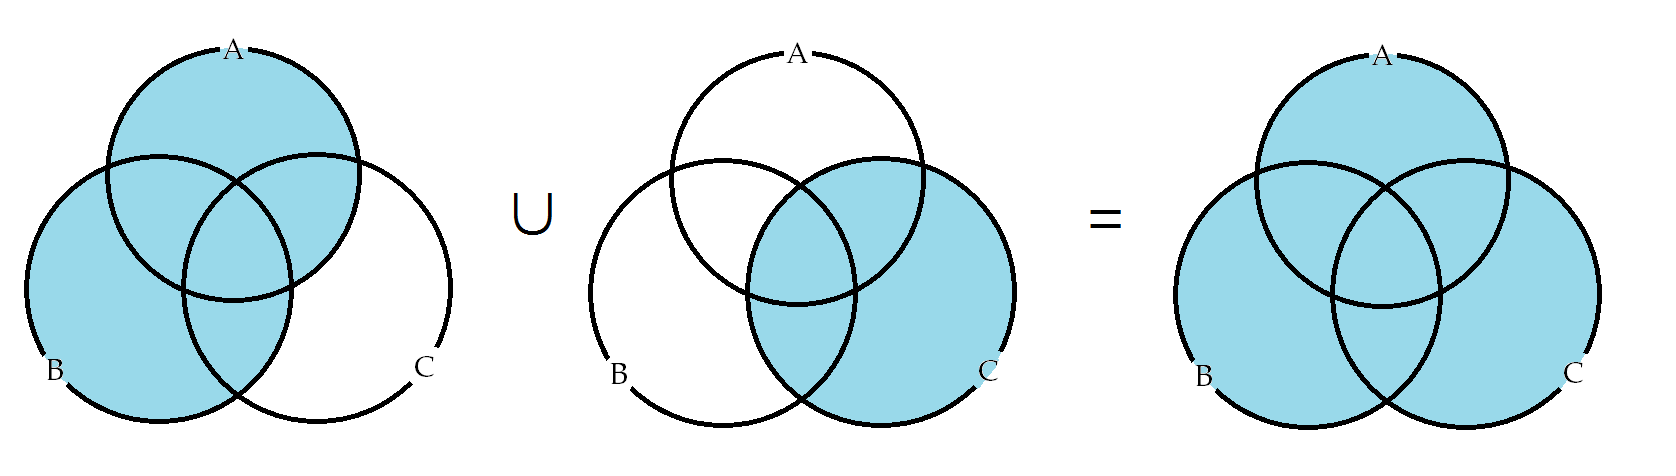
\includegraphics[width=.9\textwidth]{properties_3-1}
\par\vspace{-10pt}
\(\qquad\:A\cup B\qquad\qquad\qquad\quad\:\:C
\qquad\qquad\qquad\:\:(A\cup B)\cup C\)
\par
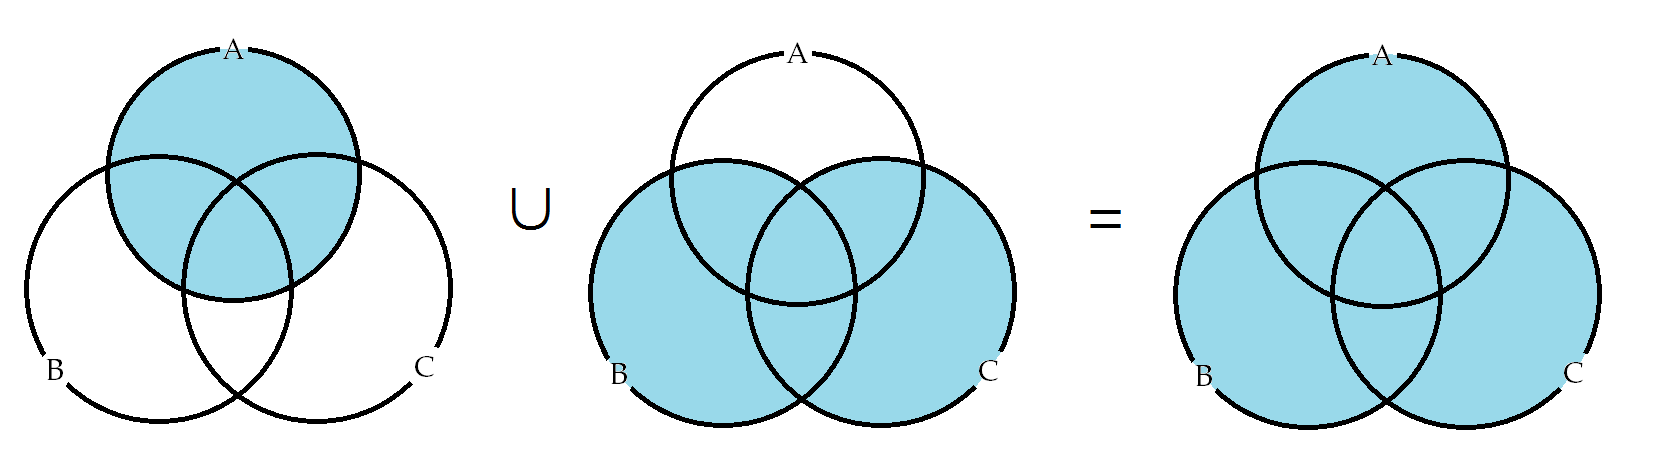
\includegraphics[width=.9\textwidth]{properties_3-2}
\par\vspace{-10pt}
\(\qquad\quad A\qquad\qquad\qquad\quad\:\:B\cup C
\qquad\qquad\quad\:\: A\cup (B\cup C)\)
\par
이다.
따라서 좌변과 우변이 같다.
\end{mdframed}
\item
\((A\cap B)\cap C=A\cap(B\cap C)\)
\begin{mdframed}
좌변과 우변을 각각 벤 다이어그램으로 표현하면
\par
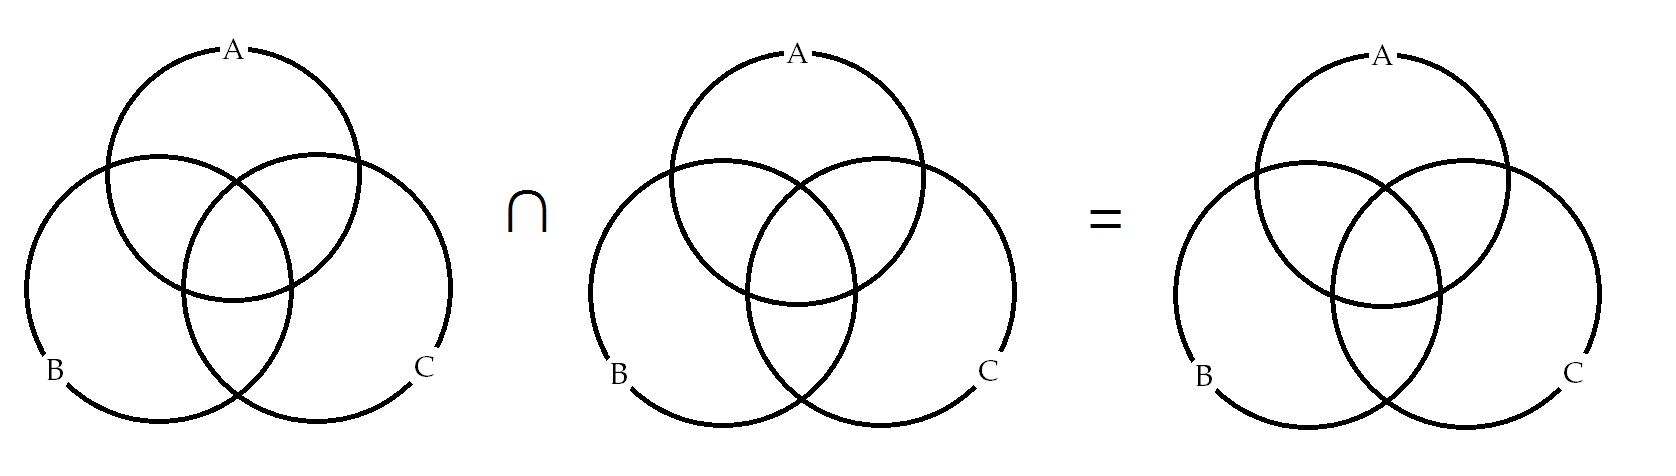
\includegraphics[width=.9\textwidth]{three_set_rule_cap}
\par\vspace{-10pt}
\(\qquad\:A\cap B\qquad\qquad\qquad\quad\:\:C
\qquad\qquad\qquad\:\:(A\cap B)\cap C\)
\par
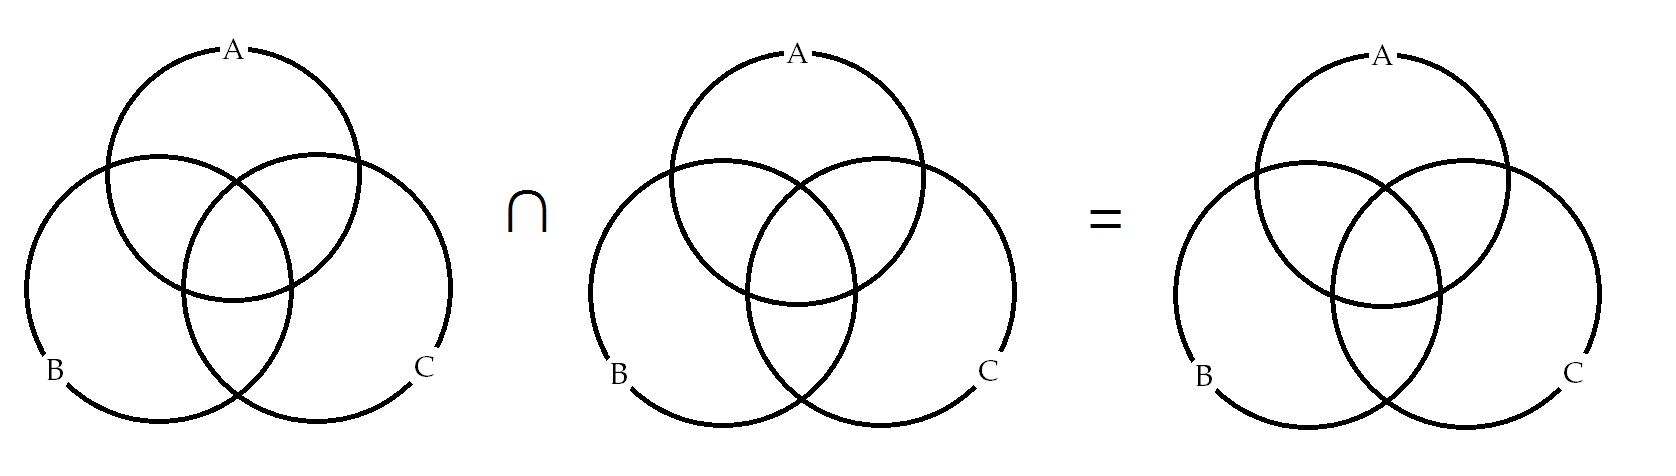
\includegraphics[width=.9\textwidth]{three_set_rule_cap}
\par\vspace{-10pt}
\(\qquad\quad A\qquad\qquad\qquad\quad\:\:B\cap C
\qquad\qquad\quad\:\: A\cap (B\cap C)\)
\par
이다.
따라서 좌변과 우변이 같다.
\end{mdframed}
\end{enumerate}
\newpage
%
\prob{분배법칙}
\begin{enumerate}\label{properties4}
\item
\(A\cup(B\cap C)=(A\cup B)\cap(A\cup C)\)
\begin{mdframed}
좌변과 우변을 각각 벤 다이어그램으로 표현하면
\par
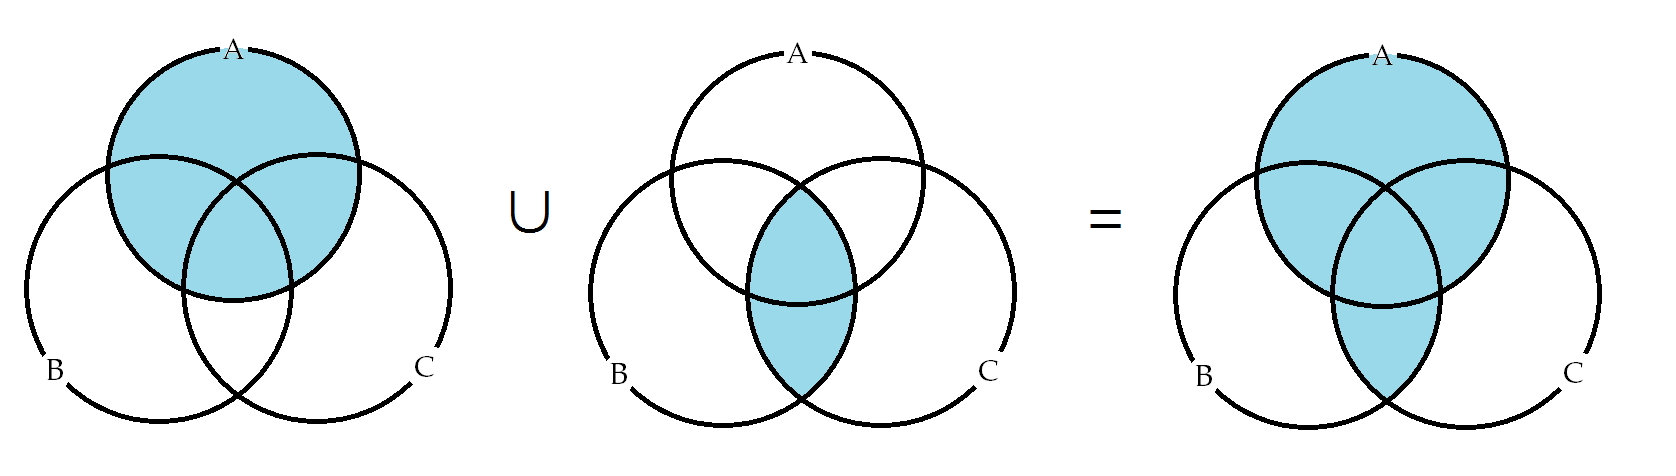
\includegraphics[width=.9\textwidth]{properties_4-1}
\par\vspace{-10pt}
\(\qquad\quad\:A\qquad\qquad\qquad\quad\:\:B\cap C
\qquad\qquad\quad\:A\cup(B\cap C)\)
\par
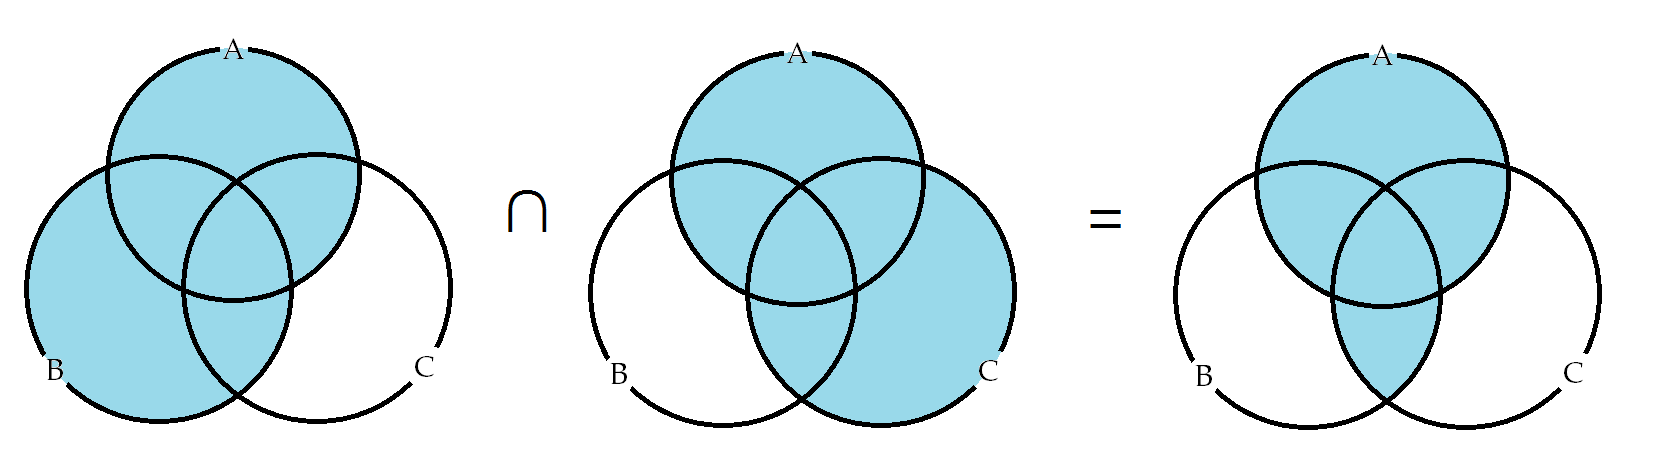
\includegraphics[width=.9\textwidth]{properties_4-2}
\par\vspace{-10pt}
\(\qquad A\cup B\qquad\qquad\qquad\:\:A\cup C
\qquad\qquad(A\cup B)\cap(A\cup C)\)
\par
이다.
따라서 좌변과 우변이 같다.
\end{mdframed}
\item
\(A\cap(B\cup C)=(A\cap B)\cup(A\cap C)\)
\begin{mdframed}
좌변과 우변을 각각 벤 다이어그램으로 표현하면
\par
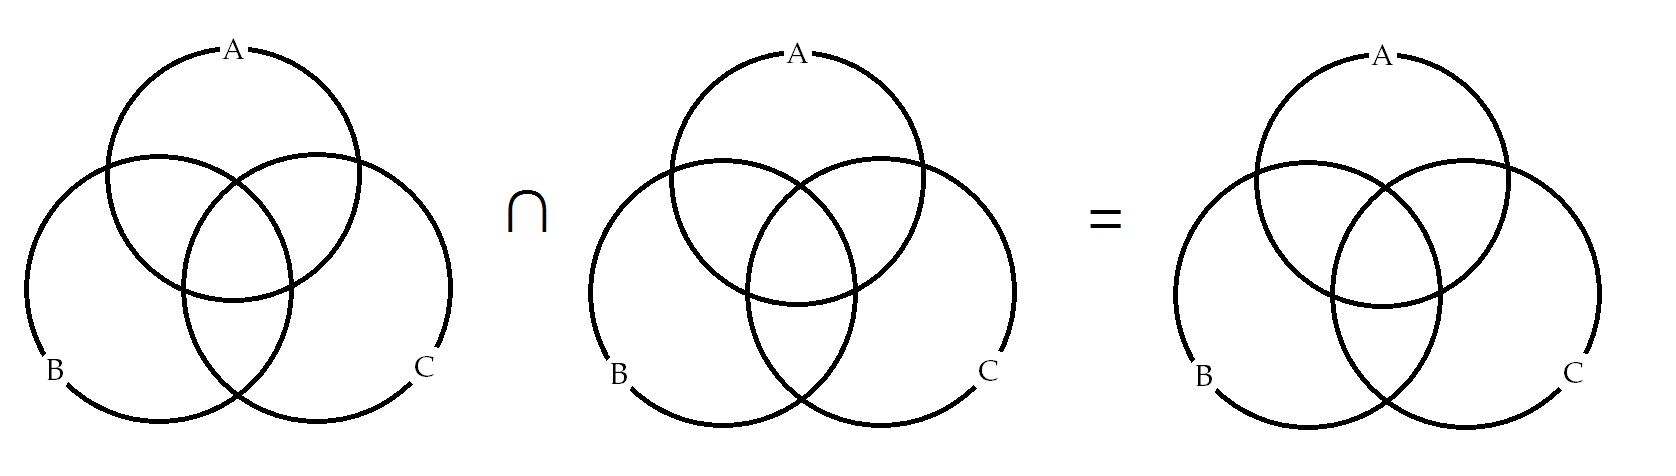
\includegraphics[width=.9\textwidth]{three_set_rule_cap}
\par\vspace{-10pt}
\(\qquad\quad\:A\qquad\qquad\qquad\quad\:\:B\cup C
\qquad\qquad\quad\:A\cap(B\cup C)\)
\par
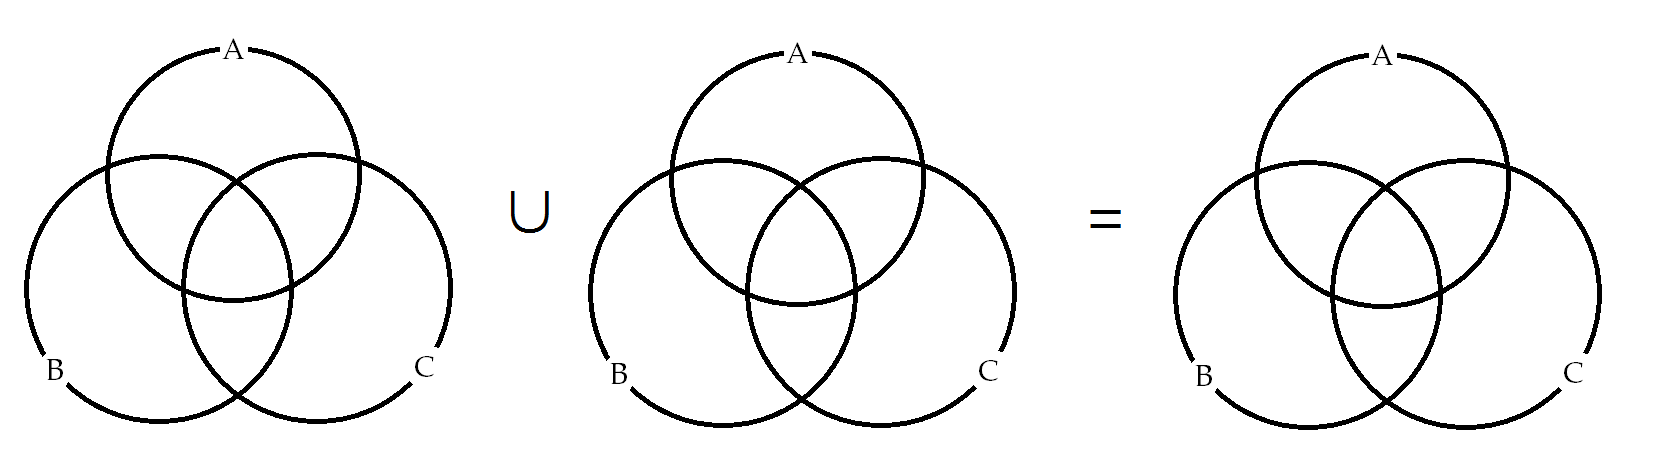
\includegraphics[width=.9\textwidth]{three_set_rule_cup}
\par\vspace{-10pt}
\(\qquad A\cap B\qquad\qquad\qquad\:\:A\cap C
\qquad\qquad(A\cap B)\cup(A\cap C)\)
\par
이다.
따라서 좌변과 우변이 같다.
\end{mdframed}
\end{enumerate}

\clearpage
%
\prob{차집합에 대한 교환법칙과 결합법칙은 성립하는지 확인하여라.}
교환법칙\::\:\(A-B\stackrel?=B-A\)\\\label{properties5}
결합법칙\::\:\(A-(B-C)\stackrel?=(A-B)-C\)
\begin{mdframed}
교환법칙 :
\par\vspace{-20pt}
\begin{center}
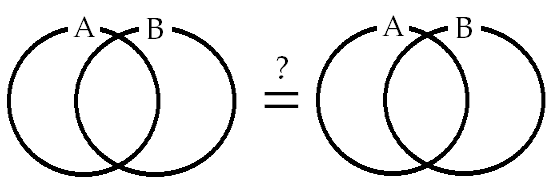
\includegraphics[width=.5\textwidth]{two_set_equality}
\par\(A-B\qquad\qquad\qquad\:\:B-A\)
\end{center}
\par\noindent
결합법칙 :
\par
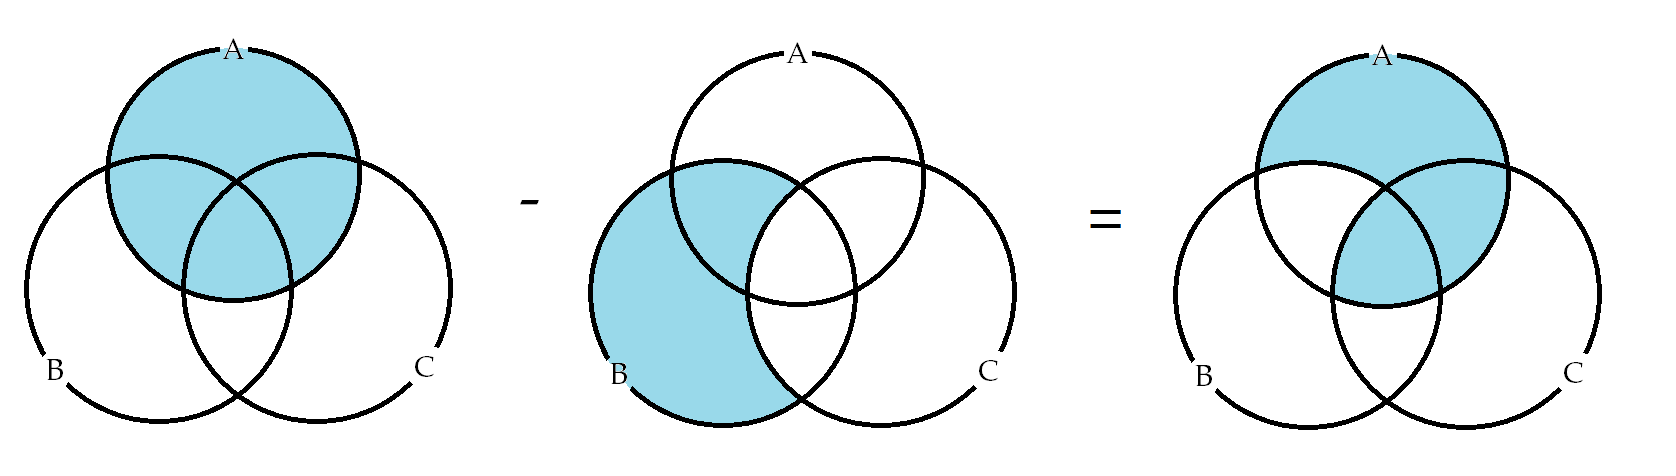
\includegraphics[width=.9\textwidth]{properties_5}
\par\vspace{-10pt}
\(\qquad\quad\:A\qquad\qquad\qquad\qquad B-C
\qquad\qquad\qquad\:A-(B-C)\)
\par
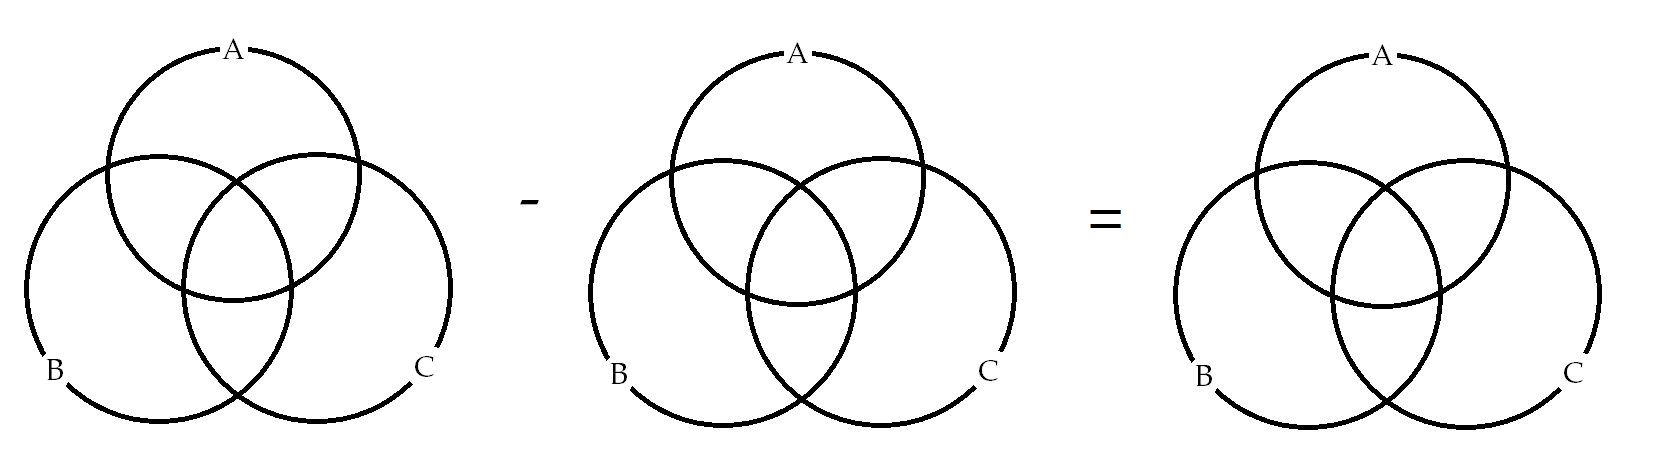
\includegraphics[width=.9\textwidth]{three_set_rule_setminus}
\par\vspace{-10pt}
\(\qquad A-B\qquad\qquad\qquad\qquad\:\: C
\qquad\qquad\qquad\quad(A-B)-C\)
\par
\end{mdframed}
\ans{
교환법칙이 (성립한다 / 성립하지 않는다.)\\
결합법칙이 (성립한다 / 성립하지 않는다.)
}
\newpage

%\vspace{-10pt}
%%
%\prob{차집합의 성질 : \(A\cap B^c=A-B\)}\label{properties6}
%\begin{mdframed}[skipabove=0pt,innertopmargin=5pt]
%좌변을 벤 다이어그램으로 표현하면
%\par
%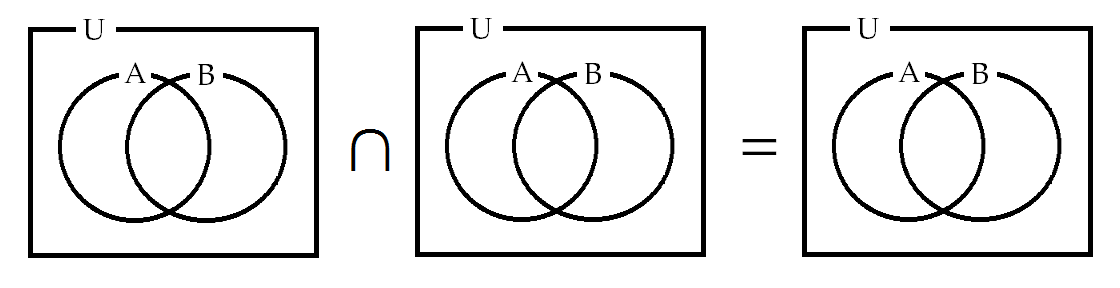
\includegraphics[width=.9\textwidth]{two_set_rule-cap}
%\par\vspace{-10pt}
%\(\qquad\qquad A\qquad\qquad\qquad\qquad\quad\:B^c
%\qquad\qquad\qquad\quad\:\:A\cap B^c\)
%\par\noindent
%이다.
%따라서 우변인 \(A-B\)와 같다.
%\end{mdframed}

%
\prob{드 모르간의 법칙}
\begin{enumerate}\label{properties7}
\item
\((A\cup B)^c=A^c\cap B^c\)
\begin{mdframed}
좌변과 우변을 각각 벤 다이어그램으로 표현하면
\par
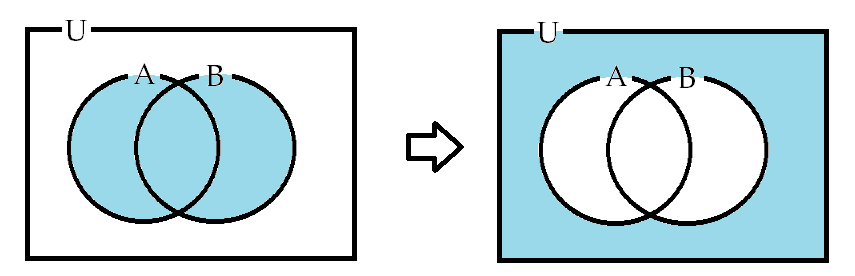
\includegraphics[width=.9\textwidth]{properties_7-1}
\par\vspace{-10pt}
\(\qquad\qquad\:\: A\cup B\qquad\qquad\qquad\qquad\qquad\quad\:\:(A\cup B)^c\)
\par
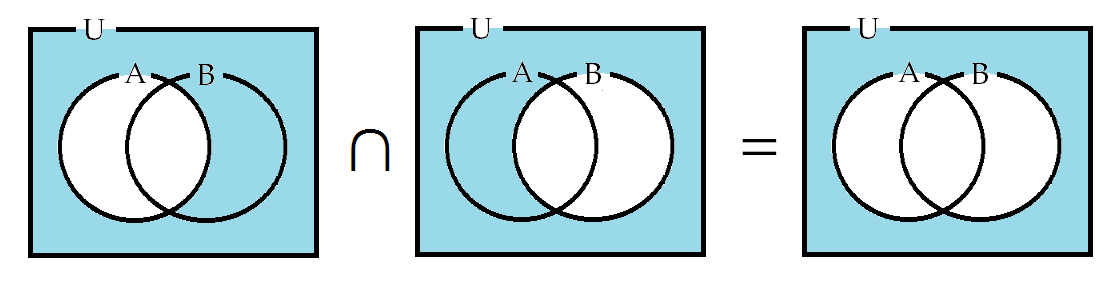
\includegraphics[width=.9\textwidth]{properties_7-2}
\par\vspace{-10pt}
\(\qquad\quad\:\:A^c\qquad\qquad\qquad\qquad B^c
\qquad\qquad\qquad A^c\cap B^c\)
\par
이다.
따라서 좌변과 우변이 같다.
\end{mdframed}
\item
\((A\cap B)^c=A^c\cup B^c\)
\begin{mdframed}
좌변과 우변을 각각 벤 다이어그램으로 표현하면
\par
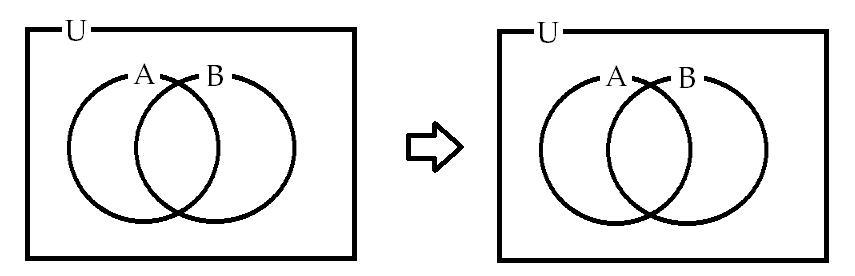
\includegraphics[width=.9\textwidth]{two_set_rule-complement}
\par\vspace{-10pt}
\(\qquad\qquad\:\: A\cap B\qquad\qquad\qquad\qquad\qquad\quad\:\:(A\cap B)^c\)
\par
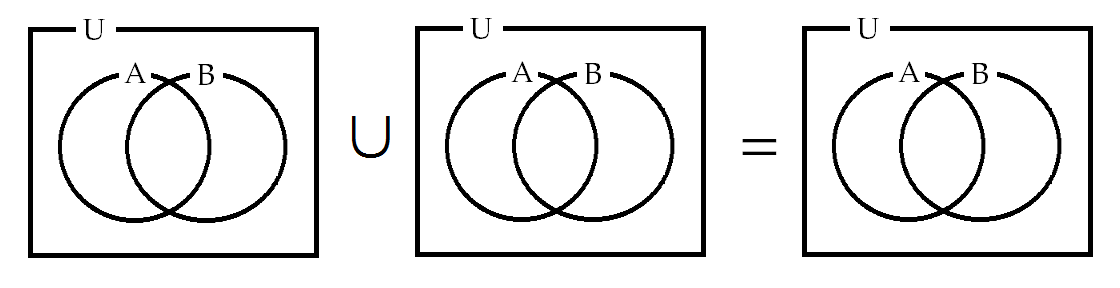
\includegraphics[width=.9\textwidth]{two_set_rule-cup}
\par\vspace{-10pt}
\(\qquad\quad\:\:A^c\qquad\qquad\qquad\qquad B^c
\qquad\qquad\qquad A^c\cup B^c\)
\par
이다.
따라서 좌변과 우변이 같다.
\end{mdframed}
\end{enumerate}

%%cardinal
\section{유한집합의 원소의 개수}

%
\begin{mdframed}
\defi{}\label{cardinal1}
집합\(A\) 의 원소의 개수는 \(n(A)\)로 나타낸다.
\end{mdframed}

%
\exam{}
\begin{enumerate}\label{cardinal2}
\item
\(n(\varnothing)=0\)이다.
\item
\(A=\{1,2,3\}\)이면 \(n(A)=3\)이다.
\item
\(B=\{x\ba x\text{는 15 이하의 짝수}\}\)이면 \(n(B)=7\)이다.
\end{enumerate}

\begin{mdframed}
%
\theo{\(n(A\cup B)=n(A)+n(B)-n(A\cap B)\)}\label{cardinal3}
\begin{center}
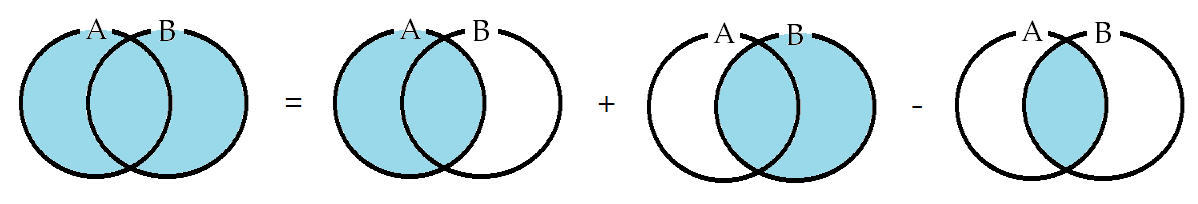
\includegraphics[width=0.9\textwidth]{cardinal_3-2}
\end{center}
\end{mdframed}

%
\exam{}\label{cardinal4}
\(n(A)=7,\:\:n(B)=4,\:\:n(A\cap B)=3\)일 때, \(n(A\cup B)\)의 값을 구하여라.
\begin{mdframed}
\(n(A\cup B)=n(A)+n(B)-n(A\cap B)=7+4-3=8\)
\end{mdframed}
\ans{\(8\)}

%
\prob{}\label{cardinal5}
\(n(A)=5,\:\:n(B)=11,\:\:n(A\cup B)=13\)일 때, \(n(A\cap B)\)의 값을 구하여라.

%
\prob{}\label{cardinal6}
\(A\cap B=\varnothing,\:\:n(A)=10,\:\:n(A\cup B)=27\)일 때, \(n(B)\)의 값을 구하여라.

%%
\section*{답}
\addcontentsline{toc}{chapter}{\protect\numberline{*}답}
\begin{multicols*}{2}

%
\an{sets3}
\begin{enumerate}
\item
집합이다.
\item
집합이 아니다.
\item
집합이다.
\item
집합이 아니다.
\item
집합이다.
\end{enumerate}

%
\an{sets4}
\begin{enumerate*}[itemjoin={,\quad}]
\item
\(\notin\)
\item
\(\in\)
\item
\(\in\)
\item
\(\notin\)
\end{enumerate*}

%
\an{sets5}
\begin{itemize}
\item
원소나열법\\
\(A=\{1,2,3,6,9,18\}\)
\item
조건제시법\\
\(A=\{x\ba x\text{는 \(18\)의 약수}\}\)
\end{itemize}

%
\an{sets6}
\begin{itemize}
\item
원소나열법\\
\(A=\{4,8,12,16,\cdots\}\)
\item
조건제시법\\
\(A=\{x\ba x\text{는 \(4\)의 배수}\}\)\\
\(A=\{4k\ba\text{k는 자연수}\}\)
\end{itemize}

%
\an{subset2}
\begin{enumerate*}[itemjoin={,\:\:}]
\item
\(A\subset B\)
\item
\(A\supset B\)
\item
\(A=B\)
\end{enumerate*}

%
\ann{subset3}\four

\columnbreak

%
\an{subset4}
\begin{center}
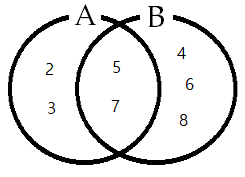
\includegraphics[width=0.2\textwidth]{subset_4}
\end{center}

%
\an{ssubset2}
\begin{enumerate}
\item
\(2\)개\\
\(\varnothing\), \(\{a\}\)
\item
\(8\)개\\
\(\varnothing\), \(\{a\}\), \(\{b\}\), \(\{c\}\),
\(\{a,b\}\), \(\{a,c\}\), \(\{b,c\}\), \(\{a,b,c\}\)
\item
\(16\)개\\
{\raggedright
\(\varnothing\), \(\{a\}\), \(\{b\}\), \(\{c\}\), \(\{d\}\),
\(\{a,b\}\), \(\{a,c\}\), \(\{a,d\}\),  \(\{b,c\}\),  \(\{b,d\}\), \(\{c,d\}\),
\(\{a,b,c\}\), \(\{a,b,d\}\), \(\{a,c,d\}\), \(\{b,c,d\}\), \(\{a,b,c,d\}\)}
\end{enumerate}

%
\an{ssubset3}
\begin{enumerate}
\item
\(32\)개
\item
\(64\)개
\end{enumerate}

%
\par\bigskip\noindent\textbf{정리 \ref{ssubset4})}\:\:\(2^k\)\par\medskip\noindent

%
\ann{ssubset5}{\(16\)개}

%
\an{ssubset7}
\begin{enumerate*}[itemjoin={,\:}]
\item \(8\)개
\item \(8\)개
\item \(4\)개
\item \(4\)개
\end{enumerate*}

%
\par\bigskip\noindent\textbf{정리 \ref{ssubset8})}\:\:\(2^{k-m}\)\par\medskip\noindent

%
\an{operations3}
\begin{enumerate}
\item
\(
A\cup B=\{1,2,3,5,7,9\}\\
A\cap B=\{3,5,7\}\\
A-B=\{1,9\}\\
B-A=\{2\}
\)
\item
\(
A\cup B=\{1,2,3,4,6,12\}\\
A\cap B=\{1,2,3,6\}\\
A-B=\varnothing\\
B-A=\{4,12\}
\)
\end{enumerate}

%
\an{operations4}
\begin{enumerate}
\item
\(\{2,4,5,6,7,8,9,10\}\)
\item
\(\{1,2,4,5,6,7,8,9,10\}\)
\end{enumerate}

%
\ann{operations6}{\(A\), \(C\)}

%
\an{operations9}
\(
A^c=\{6,7\}\\
B^c=\{2,3,5,6\}\\
A\cap B^c=\{2,3,5\}
\)

%%
%\an{operations10}
%\(
%A\cup B=\{2,3,4,5,6,7,8,10\}\\
%(A\cup B)^c=\{1,9\}\\
%A\cap B=\{2\}\\
%(A\cap B)^c=\{1,3,4,5,6,7,8,9,10\}
%\)

%
\ann{operations11}{\four}

%
\ann{properties3}{생략}

%
\ann{properties4}{생략}

%
\ann{properties5}{생략}
성립하지 않는다, 성립하지 않는다.

%%
%\ann{properties6}{생략}

%
\ann{properties7}{생략}

%
\ann{cardinal5}3

%
\ann{cardinal6}{17}

\end{multicols*}


%%
\section*{요약}
\addcontentsline{toc}{chapter}{\protect\numberline{*}요약}
\begin{enumerate}[label=\arabic*.,itemsep=15pt]
\item
집합과 원소
\begin{itemize}
\item
원소나열법\::\:\(A=\{1,3,5,7,9,\cdots\}\)
\item
조건제시법\::\:\(A=\{x\ba x\text{는 홀수}\}=\{2k-1\ba\text{k는 자연수}\}\)
\end{itemize}
\item
부분집합\\
\(A=\{2,5\}\)이면\quad
\(\underline{2\in A,\:\:5\in A},\quad
\underline{\emptyset\subset A,\:\:\{2\}\subset A,\:\:\{3\}\subset A,\:\:\{2,5\}\subset A}\).
\item
부분집합의 개수
\[n(A)=k\text{이면, \(A\)의 부분집합의 개수는 \fbox{\(2^k\)}개}\]
\item
집합의 연산
\begin{figure}[h]
\centering
        \begin{subfigure}{0.2\textwidth}
                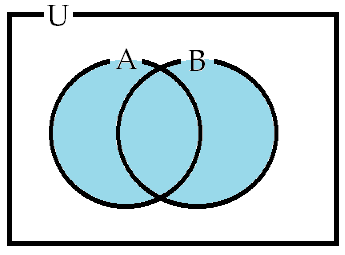
\includegraphics[width=\linewidth]{summary_4-1}
                \caption*{\(A\cup B\)}
        \end{subfigure}%
\quad
        \begin{subfigure}{0.2\textwidth}
                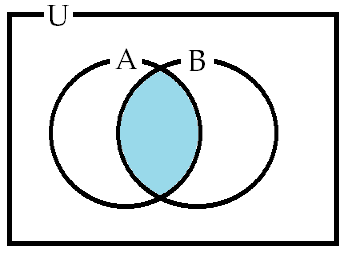
\includegraphics[width=\linewidth]{summary_4-2}
                \caption*{\(A\cap B\)}
        \end{subfigure}%
\quad
        \begin{subfigure}{0.2\textwidth}
                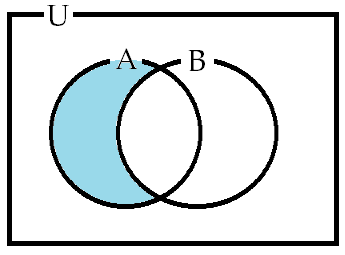
\includegraphics[width=\linewidth]{summary_4-3}
                \caption*{\(A-B\)}
        \end{subfigure}%
\quad
        \begin{subfigure}{0.2\textwidth}
                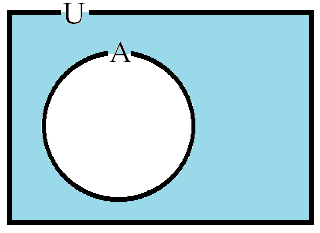
\includegraphics[width=\linewidth]{summary_4-4}
                \caption*{\(A^c\)}
        \end{subfigure}
\end{figure}
\item
집합의 연산법칙
\begin{enumerate}
\item
\(A\cup B=B\cup A,\quad A\cap B=B\cap A\)
\tabto{.6\textwidth}[교환법칙]
\item
\((A\cup B)\cup C=A\cup(B\cup C)\)
\tabto{.6\textwidth}[결합법칙]\\
\((A\cap B)\cap C=A\cap(B\cap C)\)
\item
\(A\cup(B\cap C)=(A\cup B)\cap(A\cup C)\)
\tabto{.6\textwidth}[분배법칙]\\
\(A\cap(B\cup C)=(A\cap B)\cup(A\cap C)\)
\item
\(A-B=A\cap B^c\)
\tabto{.6\textwidth}[차집합의 성질]
\item
\((A\cup B)^c=A^c\cap B^c\)
\tabto{.6\textwidth}[드 모르간의 법칙]\\
\((A\cap B)^c=A^c\cup B^c\)
\end{enumerate}
\item
유한집합의 원소의 개수
\[n(A\cup B)=n(A)+n(B)-n(A\cap B)\]
\end{enumerate}
\end{document}